\section{Environment}
\subsection{Apache Flink}
For this paper, we used Apache Flink as data processing engine. Flink is a Fast and Reliable
Large-Scale Data Processing engine. A Flink cluster can be made up from a number of physical
computation nodes or even a single host. Processing programs, written in Java or Scala, are
automatically adapted by the optimizer and runtime to execute efficient on a given setup.
\footnote{(2015) Apache Flink home. Retrieved March 20, 2015, from https://flink.apache.org/.}
The result of this adaption is the so-called Execution Graph, which is deployed. A master-node, the
Job Manager is responsible for doing so and keeping track of the the overall job execution. The job
is split up into several tasks that can be handled independant by Task Managers - the actual
computation nodes.  Depending on the physical hardware, a task manager can offer multiple processing
slots. A sketch of the processing is depicted below.

\begin{figure}
\centering
\begin{minipage}{0.5\textwidth}
  \centering
  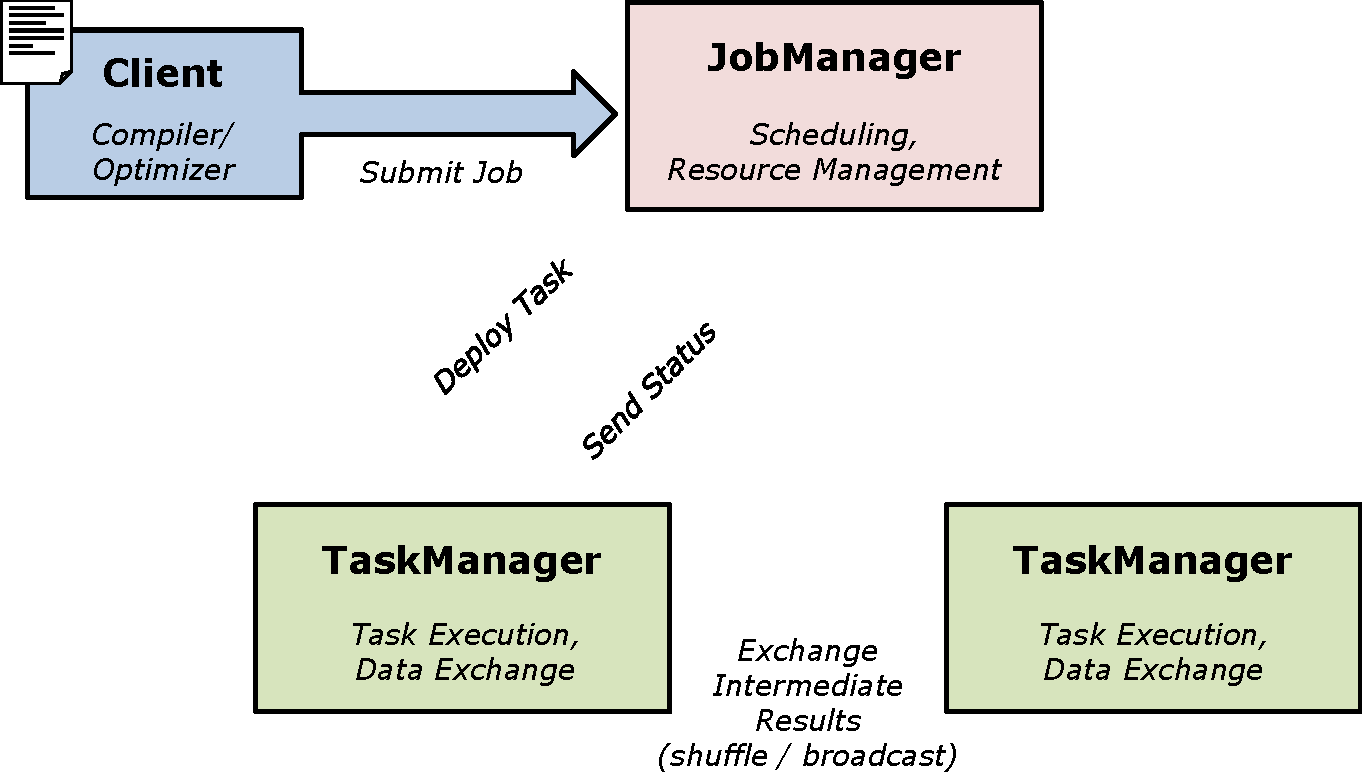
\includegraphics[width=1.0\linewidth]{graphics/ClientJmTm.pdf}
    \captionof{figure}{Sketch of Job Execution\protect\footnotemark}
  \label{fig:jobexecution}
\end{minipage}%
\begin{minipage}{0.5\textwidth}
  \centering
  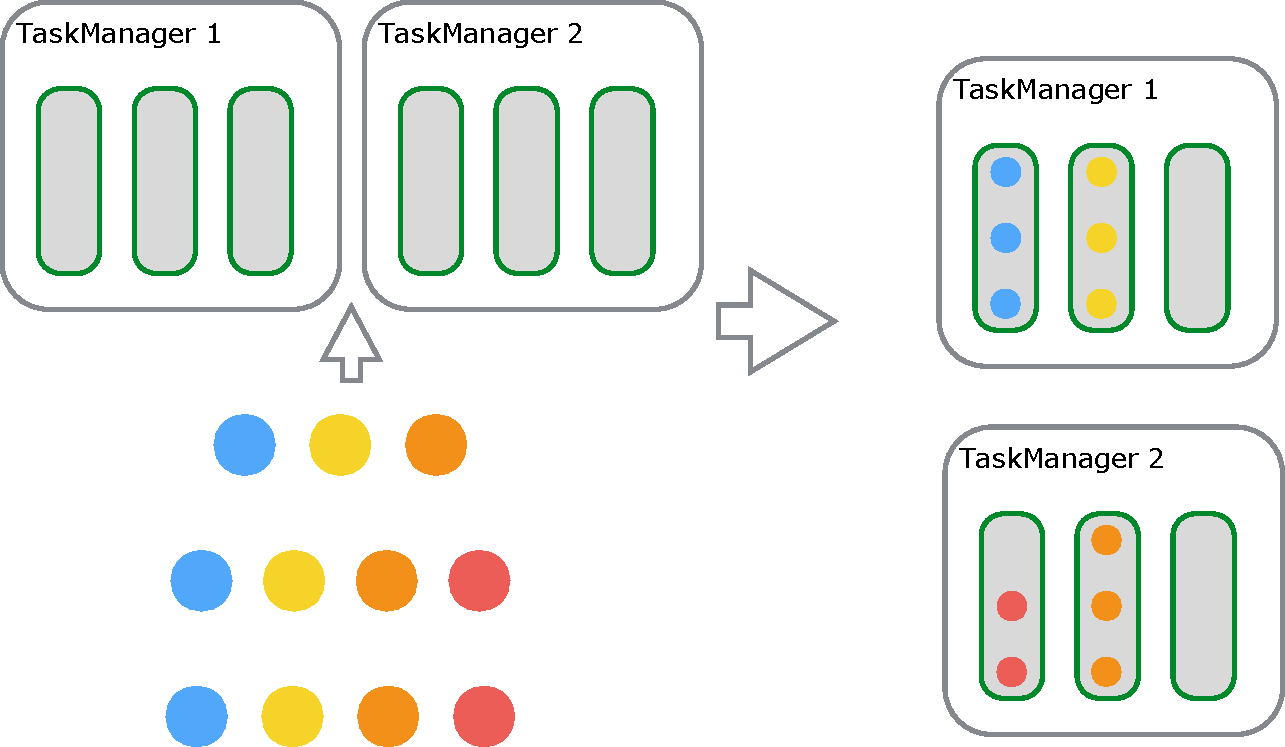
\includegraphics[width=1.0\linewidth]{graphics/slots.pdf}
    \captionof{figure}{Execution-Graph embedding to Task Managers\protect\footnotemark}
  \label{fig:embedding}
\end{minipage}
\end{figure}

\footnotetext{(2015) ClientJmTm.svg Github/Apache/Flink-master from
https://raw.githubusercontent.com/apache/flink/master/docs/img/ClientJmTm.svg.}

\footnotetext{(2015) Slots.svg Github/Apache/Flink-master from
https://raw.githubusercontent.com/apache/flink/master/docs/img/slots.svg.}

